% Copyright 2011 by Joseph Pan
%
% This file may be distributed and/or modified
%
% 1. under the LaTeX Project Public License and/or
% 2. under the GNU Public License.
%
% To compile this file, you may need:
% 1. LaTeX
% 2. Beamer
% 3. CJK

\documentclass{beamer}

% Setup appearance:

\graphicspath{{Images/}}

\mode<presentation>
{
  \usetheme{Darmstadt}
  % or ...

  \setbeamercovered{transparent}
  % or whatever (possibly just delete it)
}

% Standard packages

\usepackage[english]{babel}
\usepackage[latin1]{inputenc}
\usepackage{times}
\usepackage[T1]{fontenc}


% CJK packages
\usepackage{xeCJK}
\setCJKmainfont{WenQuanYi Micro Hei Mono}% 文泉驿等宽微米黑


% Setup TikZ

\usepackage{tikz}
\usetikzlibrary{arrows}
\tikzstyle{block}=[draw opacity=0.7,line width=1.4cm]

% Graphix
\usepackage{graphicx}

% Author, Title, etc.

\title[AES Parallel Computing]
{基于GPU异构平台的AES并行计算}

\author[Edwin Ho] % (optional, use only with lots of authors)
{何振忠}

\institute[South China Normal University(SCNU)] % (optional, but mostly needed)
{
  School of Computer\\
  South China Normal University
}

% - Use the \inst command only if there are several affiliations.
% - Keep it simple, no one is interested in your street address.

\date[WABI 2013]
{6/3, 2013}

% Delete this, if you do not want the table of contents to pop up at
% the beginning of each subsection:
\begin{comment}
\AtBeginSubsection[]
{
          \begin{frame}<beamer>{Outline}
              \tableofcontents[currentsection,currentsubsection]
                    \end{frame}
}
\end{comment}

% The main document

\begin{document}

\begin{frame}
  \titlepage
\end{frame}

\begin{frame}{Mind Map}
  \begin{figure}
    \raggedright
    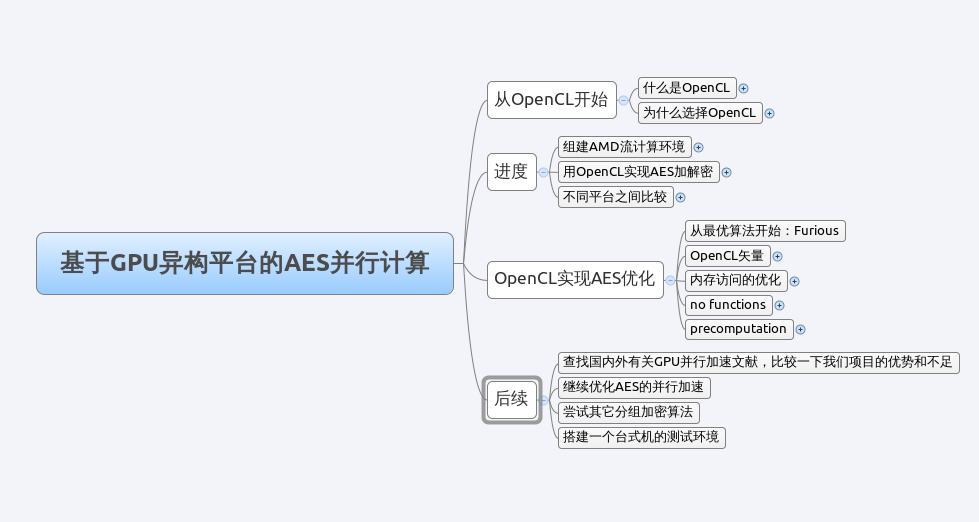
\includegraphics[width=11cm]{mindmap.png}
  \end{figure}
\end{frame}

\begin{frame}{Outline}
  \tableofcontents
\end{frame}

\section{从OpenCL开始}

\subsection{什么是OpenCL}

\begin{frame}{Open Computing Language}
    OpenCL为异构平台提供一个编写程序,特别是并行程序的开放框架标准。\\
    \begin{center}
    
\includegraphics[width=10cm]{Khronos.png}
    \end{center}
\end{frame}

\begin{frame}{组成}
    OpenCL由两部分组成:
    \begin{itemize}
          \item 编写内核程序的语言\\
                OpenCL C 是基于 ISO/IEC 9899:1999 C 标准做了一定的扩展和限制.
                \begin{columns}[t]
                \column{.5\textwidth}
                        \centering
                        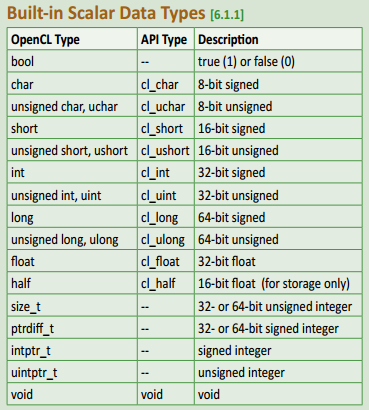
\includegraphics[width=5cm]{scalarType.png}
                \column{.5\textwidth}
                        \centering
                        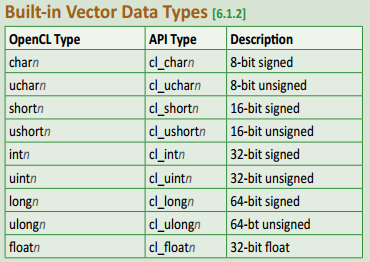
\includegraphics[width=5cm]{vectorType.png}
                \end{columns}
    \end{itemize}
\end{frame}

\begin{frame}{组成}
    OpenCL由两部分组成:
    \begin{itemize}
          \item 定义并控制平台的API\\
                适用于各种类型异构处理器的坐标数据和基于任务并行计算
                API.
                \begin{center}
                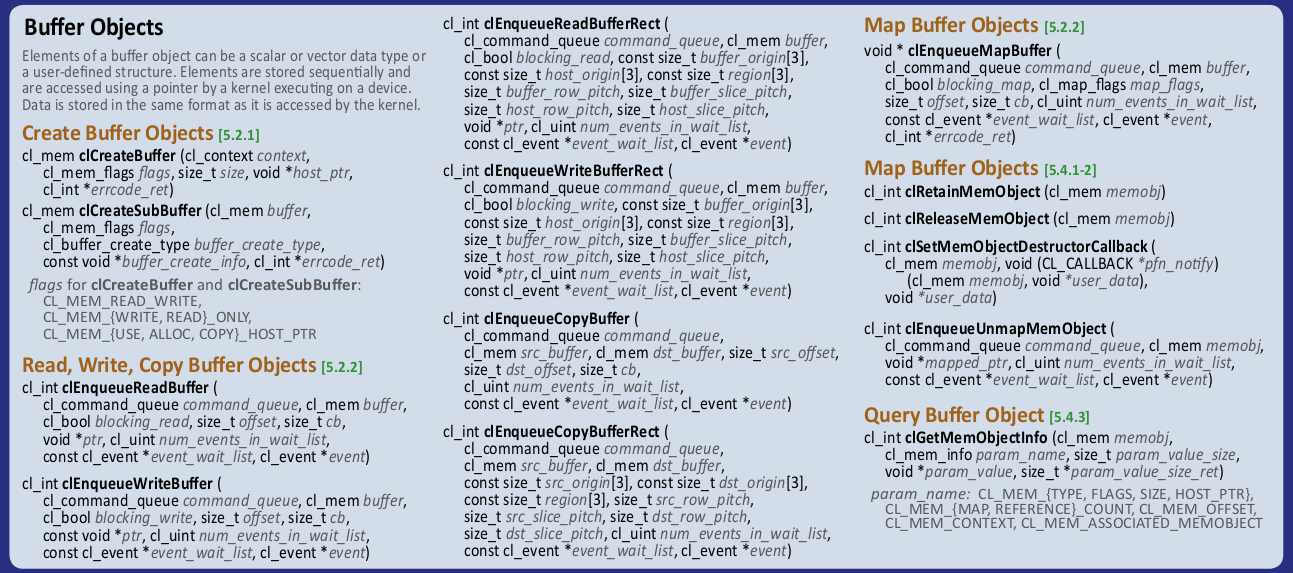
\includegraphics[width=10cm]{API.png}
                \end{center}

    \end{itemize}
\end{frame}

\subsection{为什么选择OpenCL}
\begin{frame}{OpenCL可以充分利用设备的并行性}
    \begin{itemize}
          \item GPU的运算核心数量要远远超过高端CPU的核心数量
          \item GPU是通过大量并行线程之间交织运算隐藏全局访问的延迟
                \begin{center}
                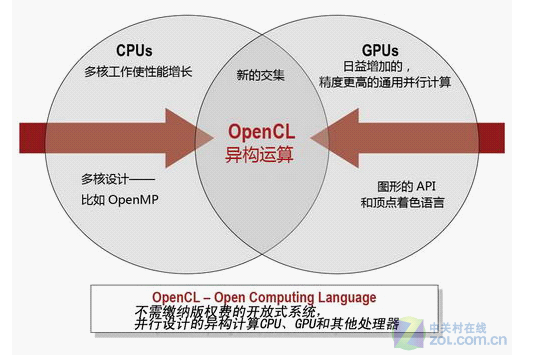
\includegraphics[width=9cm]{parallel.png}
                \end{center}
    \end{itemize}       
\end{frame}

\begin{frame}{OpenCL为程序员提供了平台独立性}
     问题:不同平台,不同厂商,不同产品型号的GPU往往有着不同的架构。\\
     解决:OpenCL支持各种各样的并行处理器的组合平台。
     \begin{center}
     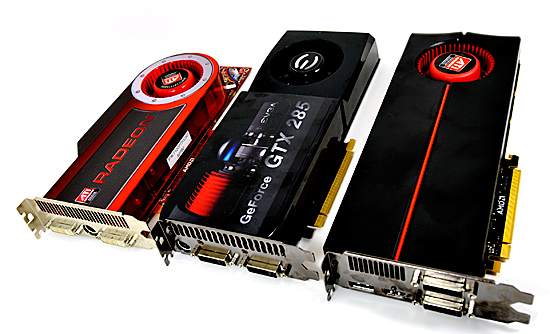
\includegraphics[width=10cm]{hardware.jpg}
     \end{center}
\end{frame}

\section{进度}

\subsection{组建AMD流计算环境}

\begin{frame}{Windows}
     \begin{itemize}
     \item 安装ATI driver
     \item AMD Stream SDK
     \item IDE: MS Visual Studio 2010
     \end{itemize}
     \centering
     
\includegraphics[width=5cm]{windows.jpg}
\end{frame}


\begin{frame}{Linux}
     \begin{itemize}
     \item 安装ATI driver
     \item AMD Stream SDK
     \item 将库文件路径添加到环境变量中
     \end{itemize}
     \centering
     
\includegraphics[width=5cm]{linux.jpg}
\end{frame}

\subsection{基于GPU上加解密}

\begin{frame}{AES Encryption}
在CPU完成密钥扩展后,将明文和扩展密钥复制到GPU上进行AES加密。

\end{frame}

\subsection{不同平台之间比较}

\begin{frame}{用相同的密钥加密不同长度的明文}
   \begin{columns}[t]
      \column{.5\textwidth}
      \centering
      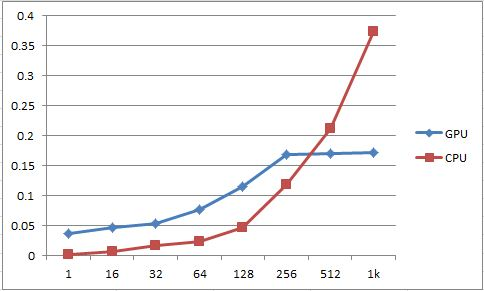
\includegraphics[width=6cm]{graph1.jpg}
      \column{.5\textwidth}
      \centering
      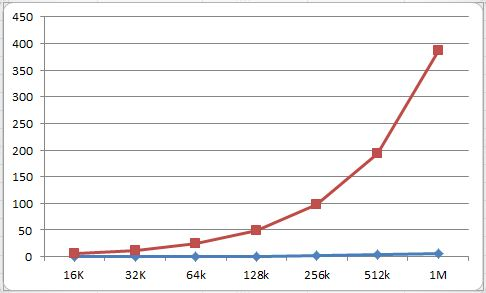
\includegraphics[width=6cm]{graph2.jpg}
   \end{columns}
\end{frame}

\begin{frame}{N个明文,K个密钥}
   \begin{center}
      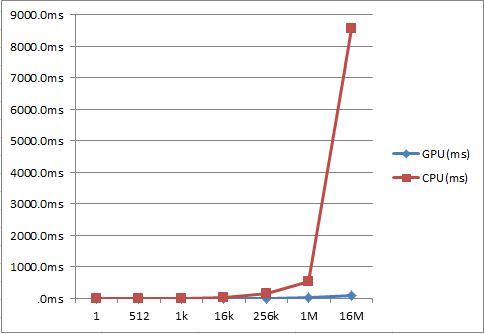
\includegraphics[width=8cm]{graph3.jpg}
   \end{center}
\end{frame}

\section{AES优化}

\subsection{从最优算法开始}
\begin{frame}{Furious}
\huge Furious
\begin{figure}

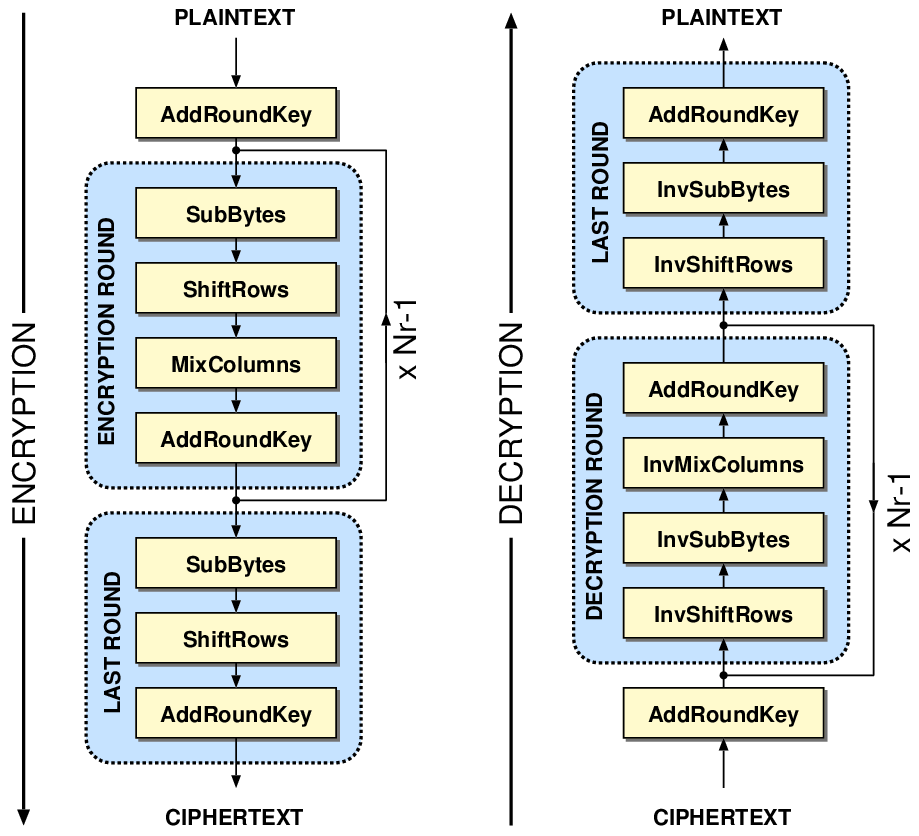
\includegraphics[width=7cm]{rijndael.png}
\end{figure}
\end{frame}

\subsection{OpenCL矢量}

\begin{frame}{OpenCL矢量}
矢量化允许一个线程同时执行多个操作。\\
矢量化在AMD的GPU上效果更明显。

\end{frame}

\subsection{内存访问的优化}

\begin{frame}{Global Memory}
Global Memory的访存模式也会在很大程度上影响程序的性能。\\
2种需要把数据写回Global Menory的情况:
   \begin{itemize}
   \item Kernel需要保存作为输出的数据
   \item 需要在Group之间交换数据   
   \end{itemize}
\end{frame}

\begin{frame}{Local Memory}
  Local Memory是指在 GPU上对每个 Thread Group有一块可以进行快速访问的内存.
\end{frame}

\subsection{No Functions}

\begin{frame}{No Functions}
   将AddRoundKey、SubBytes、ShiftRows、MixColumns四个操作都写到循环里,
   省去函数的调用时间。
   \centering
   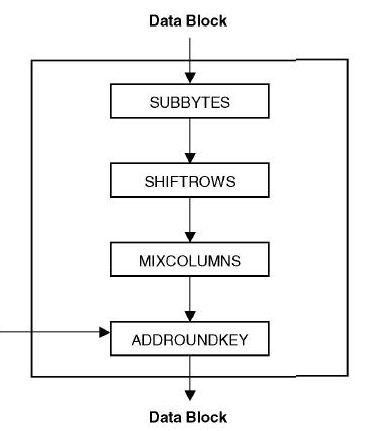
\includegraphics[width=6cm]{round.jpg}
\end{frame}

\subsection{Precomputation}

\begin{frame}{Precomputation}
   将全部密钥都做完密钥扩展后复制到GPU。
\end{frame}

\section{后续}

\subsection{后续工作}
\begin{frame}{No.1}
  \begin{itemize}
  \item 查找国内外有关GPU并行加速运算的文献,比较一下我们的优劣和不足。
  \end{itemize}
\end{frame}

\begin{frame}{No.2}
  \begin{itemize}
  \item 继续优化AES的并行加速
  \end{itemize}
  \begin{figure}
    \raggedright
    
\includegraphics[width=5cm]{aes-logo.jpg}
  \end{figure}
\end{frame}

\begin{frame}{No.3}
  \begin{itemize}
  \item  尝试其它分组加密算法
  \end{itemize}
  \begin{center}
    
\includegraphics[width=8cm]{blockcipher.jpg}
    \end{center}
\end{frame}

\begin{frame}{No.4}
  \begin{itemize}
  \item  搭建一个台式机的测试环境
  \end{itemize}
\end{frame}

\section{End}

\begin{frame}{End}
  \begin{center}
    \alert{\Huge Thank You!}
  \end{center}
  
\end{frame}

\end{document}